\begin{frame}{Struttura di lavoro}
    \centering
    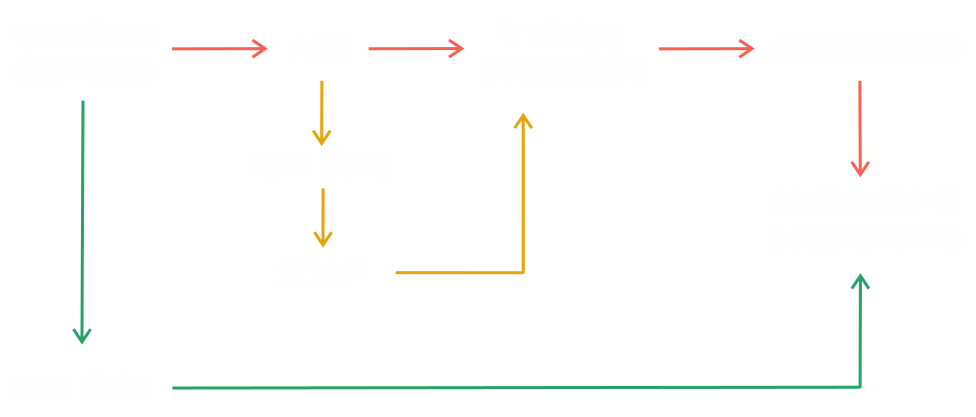
\includegraphics[scale=1.5]{invnobg/schema-lavoro - Selection.png}
\end{frame}


\subsection{SOAP} %----------------------------------------------------------------------------------------------------------------------------


\begin{frame}{SOAP}
    \begin{columns}[c]        
        % Colonna Sinistra: Testo
        \begin{column}{0.48\textwidth}
        
        -----
        
        \end{column}
        % Colonna Destra: Due immagini incolonnate
        \begin{column}{0.48\textwidth}
        
            \centering
            %\includegraphics[height=0.32\paperheight, keepaspectratio]{images/.png}
            
            \vspace{0.4cm} % Spazio verticale tra le due immagini
            
            %\includegraphics[height=0.32\paperheight, keepaspectratio]{images/.png}
            
        \end{column}
    \end{columns}
\end{frame}


\subsection{Addestramento GAP} %----------------------------------------------------------------------------------------------------------------------------


\begin{frame}{GAP}
    \begin{columns}[c]        
        % Colonna Sinistra: Testo
        \begin{column}{0.48\textwidth}
        
        -----
        
        \end{column}
        % Colonna Destra: Due immagini incolonnate
        \begin{column}{0.48\textwidth}
        
            \centering
            %\includegraphics[height=0.32\paperheight, keepaspectratio]{images/.png}
            
            \vspace{0.4cm} % Spazio verticale tra le due immagini
            
            %\includegraphics[height=0.32\paperheight, keepaspectratio]{images/.png}
            
        \end{column}
    \end{columns}
\end{frame}

\begin{frame}{GPR}
    \begin{columns}[c]        
        % Colonna Sinistra: Testo
        \begin{column}{0.48\textwidth}
        
        -----
        
        \end{column}
        % Colonna Destra: Due immagini incolonnate
        \begin{column}{0.48\textwidth}
        
            \centering
            %\includegraphics[height=0.32\paperheight, keepaspectratio]{images/.png}
            
            \vspace{0.4cm} % Spazio verticale tra le due immagini
            
            %\includegraphics[height=0.32\paperheight, keepaspectratio]{images/.png}
            
        \end{column}
    \end{columns}
\end{frame}


\subsection{Simulazione} %-------------------------------------------------------------------------------------------------------------------


\begin{frame}{Simulazione NVE}
    \begin{columns}[c]        
        % Colonna Sinistra: Testo
        \begin{column}{0.48\textwidth}
        
        -----
        
        \end{column}
        % Colonna Destra: Due immagini incolonnate
        \begin{column}{0.48\textwidth}
        
            \centering
            %\includegraphics[height=0.32\paperheight, keepaspectratio]{images/.png}
            
            \vspace{0.4cm} % Spazio verticale tra le due immagini
            
            %\includegraphics[height=0.32\paperheight, keepaspectratio]{images/.png}
            
        \end{column}
    \end{columns}
\end{frame}

\begin{frame}{ZBL}
    \begin{columns}[c]        
        % Colonna Sinistra: Testo
        \begin{column}{0.48\textwidth}
        
        -----
        
        \end{column}
        % Colonna Destra: Due immagini incolonnate
        \begin{column}{0.48\textwidth}
        
            \centering
            %\includegraphics[height=0.32\paperheight, keepaspectratio]{images/.png}
            
            \vspace{0.4cm} % Spazio verticale tra le due immagini
            
            %\includegraphics[height=0.32\paperheight, keepaspectratio]{images/.png}
            
        \end{column}
    \end{columns}
\end{frame}

\begin{frame}{Simulazione con algoritmo di Metropolis}
    \begin{columns}[c]        
        % Colonna Sinistra: Testo
        \begin{column}{0.48\textwidth}
        
        -----
        
        \end{column}
        % Colonna Destra: Due immagini incolonnate
        \begin{column}{0.48\textwidth}
        
            \centering
            %\includegraphics[height=0.32\paperheight, keepaspectratio]{images/.png}
            
            \vspace{0.4cm} % Spazio verticale tra le due immagini
            
            %\includegraphics[height=0.32\paperheight, keepaspectratio]{images/.png}
            
        \end{column}
    \end{columns}
\end{frame}